\chapter{Electronics Essentials} \label{electronics_essentials}

This beginner's guide introduces the essential components and circuit-building concepts
you will use throughout this workshop. We will cover the breadboard, LEDs, current-limiting
resistors, pushbuttons, jumper wires, and fundamental electrical safety. Later projects will
introduce additional modules---such as addressable RGB LEDs, rotary encoders, speakers, OLED
displays, and motion sensors---which connect using these same breadboard rows and power rails.

\section{The Breadboard: Your Circuit's Foundation}

\subsection{What is a breadboard?}
A breadboard is a reusable platform for prototyping electronic circuits without soldering.
It contains a grid of spring-clip holes into which component leads and jumper wires are
inserted to make electrical connections.

\begin{figure}[H]
    \centering
    \maybeincludegraphics[width=.85\linewidth]{electronics_preamble/breadboard_illustration.png}
    \caption{The workshop breadboard with the Seeed XIAO ESP32-C3 microcontroller seated.}
    \label{fig:breadboard_overview}
\end{figure}

\subsection{Understanding the layout}

\subsubsection{Numbered columns (Bus Strips)}
The main area of the breadboard is divided into lettered rows (labeled A through J) and numbered
columns (labeled 1 to 30):
\begin{itemize}
    \item On the bottom half, holes \textbf{A}, \textbf{B}, \textbf{C}, \textbf{D}, and \textbf{E} in the
    \textbf{same numbered column} are connected together internally by a vertical metal clip (a \textit{bus strip}).
    For example, placing two component leads in \textbf{A10} and \textbf{C10} connects them together because both
    share column 10.
    \item On the top half, holes \textbf{F}, \textbf{G}, \textbf{H}, \textbf{I}, and \textbf{J} in the
    \textbf{same numbered column} are likewise connected together.
    \item \textbf{Adjacent column numbers are NOT connected.} Column 10 is completely separate from Column 11.
\end{itemize}

\subsubsection{The center divider}
A plastic trench separates rows A--E from rows F--J. The two sides are \textbf{electrically isolated}
unless you connect a jumper wire across the gap. The microcontroller straddles this center trench so that
its bottom pins (in row D) and top pins (in row H) connect to separate 5-hole bus strips.

\subsubsection{Power rails}
Along the top and bottom edges run long horizontal strips called \textbf{power rails}:
\begin{itemize}
    \item \textbf{Positive rail (+, red line):} Used to distribute power (3.3V) across the board.
    \item \textbf{Ground rail (--, blue line):} Used as the common ground (GND) return path.
\end{itemize}
All holes along the same rail are connected horizontally across all columns. Once your microcontroller is seated, you
will run jumper wires from its \textbf{3V3} and \textbf{GND} pins to these rails to power your circuits.

\begin{tcolorbox}[colback=blue!5!white,colframe=blue!40!black]
    \textbf{Breadboard summary:} Holes in the \textbf{same numbered column} on the \textbf{same side} of the
    center divider (e.g., A10 through E10) are connected together. Holes in different numbered columns, or on
    opposite sides of the center divider, are separated until you connect them with a component or jumper wire.
\end{tcolorbox}


\section{LEDs: Lighting Up Your Circuits}

\subsection{What is an LED?}
An LED (Light-Emitting Diode) is a semiconductor device that produces light when electric current flows
through it in the correct direction.

\subsection{Polarity}
LEDs are \textbf{polarized}---electricity can only flow through them in one direction:
\begin{itemize}
    \item \textbf{Anode (+):} The longer leg. Connects toward the positive voltage source (microcontroller GPIO pin).
    \item \textbf{Cathode (--):} The shorter leg. Connects toward Ground (GND). If the legs have been trimmed, look for the \textbf{flat edge} on the plastic rim of the LED casing on the cathode side.
\end{itemize}

\begin{figure}[H]
\centering
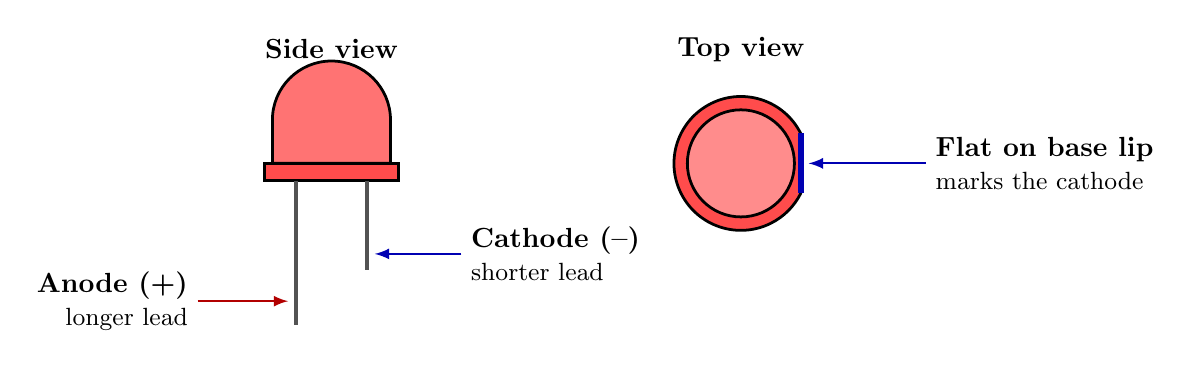
\begin{tikzpicture}[x=1cm,y=1cm,>=latex]
    % Side view: the unequal lead lengths are deliberately exaggerated.
    \node[font=\bfseries] at (-2.2,1.45) {Side view};
    \fill[red!55,draw=black,line width=1pt]
        (-2.95,0) -- (-2.95,0.55) arc[start angle=180,end angle=0,radius=0.75]
        -- (-1.45,0) -- cycle;
    \fill[red!70,draw=black,line width=1pt] (-3.05,-0.22) rectangle (-1.35,0);
    \draw[line width=1.6pt,gray!65!black] (-2.65,-0.22) -- (-2.65,-2.05);
    \draw[line width=1.6pt,gray!65!black] (-1.75,-0.22) -- (-1.75,-1.35);

    \draw[->,thick,red!70!black] (-3.9,-1.75) -- (-2.75,-1.75);
    \node[anchor=east,align=right] at (-3.9,-1.75)
        {\textbf{Anode (+)}\\\small longer lead};
    \draw[->,thick,blue!70!black] (-0.55,-1.15) -- (-1.65,-1.15);
    \node[anchor=west,align=left] at (-0.55,-1.15)
        {\textbf{Cathode (--) }\\\small shorter lead};

    % Top view: the dome is round; only the wider base lip has a small flat.
    \node[font=\bfseries] at (3.0,1.45) {Top view};
    \fill[red!70,draw=black,line width=1pt]
        (3.76,0.38)
        arc[start angle=26.6,end angle=333.4,radius=0.85]
        -- cycle;
    \fill[red!45,draw=black,line width=1pt] (3.0,0) circle[radius=0.68];
    \draw[line width=2pt,blue!70!black] (3.76,-0.38) -- (3.76,0.38);
    \draw[->,thick,blue!70!black] (5.35,0) -- (3.86,0);
    \node[anchor=west,align=left] at (5.35,0)
        {\textbf{Flat on base lip}\\\small marks the cathode};
\end{tikzpicture}
\caption{Use either clue to identify LED polarity: the cathode has the shorter lead and the flat edge.}
\label{fig:led_polarity}
\end{figure}

\subsection{Current-limiting resistor}
LEDs have very little internal resistance. If connected directly between power and ground, too much current
will flow, destroying the LED and potentially damaging the microcontroller pin.

You must \textbf{always connect a resistor in series} with an LED. ``In series'' means the current must travel
through one single path: from the pin, through the LED, through the resistor, and into ground (or vice versa).
In this kit, we use a \textbf{220\si{\ohm}} resistor for the LED.


\section{Resistors: Controlling Current Flow}

\subsection{What is a resistor?}
A resistor is a passive component that resists and limits the flow of electric current. Resistors protect
sensitive components (like LEDs) and help create reference voltages for analog sensors. Resistors have
\textbf{no polarity}---they can be installed in either orientation without affecting the circuit.

\subsection{Resistance values and identification}
Resistance is measured in ohms (\si{\ohm}) and kilohms (\SI{1}{\kilo\ohm} = \SI{1000}{\ohm}). The resistance
value is indicated by colored bands around the body of the resistor.

% Telling the 220 ohm and 10k ohm resistors apart. The resistors are drawn with
% TikZ rather than photographed because the band colors have to stay readable
% when the guide is printed in a classroom.
\definecolor{bodymetal}{HTML}{9FC2E8}
% xcolor's brown is a light tan that reads as gold next to the other bands.
\definecolor{bandbrown}{HTML}{7B4A12}

% \resistorglyph{band 1}{band 2}{band 3}{band 4}{band 5}
% The kit's resistors carry one band on each end bulge and three across the
% middle, all at roughly even spacing, so the geometry here is fixed.
\newcommand{\resistorglyph}[5]{%
\begin{tikzpicture}[x=1cm, y=1cm]
    \draw[line width=1pt, gray!50!black] (-0.5,0.3) -- (2.8,0.3);
    \draw[fill=bodymetal, draw=black!55] (0.24,0.04) rectangle (2.06,0.56);
    \draw[fill=bodymetal, draw=black!55, rounded corners=3pt] (0.02,0) rectangle (0.46,0.6);
    \draw[fill=bodymetal, draw=black!55, rounded corners=3pt] (1.84,0) rectangle (2.28,0.6);
    \fill[#1] (0.16,0.01) rectangle (0.32,0.59);
    \fill[#2] (0.62,0.05) rectangle (0.78,0.55);
    \fill[#3] (1.07,0.05) rectangle (1.23,0.55);
    \fill[#4] (1.52,0.05) rectangle (1.68,0.55);
    \fill[#5] (1.98,0.01) rectangle (2.14,0.59);
\end{tikzpicture}%
}

% \resistorcell{value}{band 1}{band 2}{band 3}{band 4}{band 5}{caption}
\newcommand{\resistorcell}[7]{%
\begin{tabular}{c}
    \textbf{#1} \\[4pt]
    \resistorglyph{#2}{#3}{#4}{#5}{#6} \\[2pt]
    \small #7
\end{tabular}%
}

\begin{tcolorbox}[colback=yellow!10!white,colframe=yellow!50!black]
    \textbf{Which resistor is which?} Both resistors are small and blue with five evenly spaced
    colored bands, and nothing is printed on them. You do not need to figure out which end to read
    from---just count the \textbf{red} bands. The \textbf{220\si{\ohm}} resistor has \textbf{two red
    bands next to each other}, and the \textbf{10\si{\kilo\ohm}} resistor has \textbf{exactly one red
    band}. Swapping the two will not damage anything, but the circuit will not behave the way this
    project describes, so ask an instructor if you are not sure.

    \medskip
    \centering
    \begin{tabular}{c @{\hspace{3em}} c}
        \resistorcell{220\si{\ohm}}{red}{red}{black}{black}{bandbrown}{two red bands} &
        \resistorcell{10\si{\kilo\ohm}}{bandbrown}{black}{black}{red}{bandbrown}{one red band}
    \end{tabular}
\end{tcolorbox}



\section{Buttons: User Input} \label{button_basics}

\subsection{What is a pushbutton?}
A pushbutton is a momentary switch that completes a connection when pressed and breaks it when released.
The buttons in your kit have four pins arranged in two connected pairs.

\begin{figure}[H]
\centering
    \maybeincludegraphics[width=.8\linewidth]{electronics_preamble/button_illustration.png}
    \caption{Pushbutton pin arrangement: the two pins on each side are internally joined.}
    \label{fig:button_pinout}
\end{figure}

\subsection{Understanding the 4-pin connection}
As shown in Figure \ref{fig:button_pinout}, the two pins on the top edge are permanently joined internally,
and the two pins on the bottom edge are permanently joined internally. Pressing the button bridges the gap
between the top pair and the bottom pair. When placing the button across rows on the breadboard, ensure your
two circuit connections go to opposite pairs so pressing the button closes the circuit.

\subsection{Internal pull-up resistors}
When a button is not pressed, an input pin would otherwise be left ``floating'' (unconnected), picking up
electrical noise. The ESP32-C3 microcontroller has built-in \textbf{pull-up resistors} that can be enabled
in MicroPython code. This pulls the pin HIGH (3.3V) when idle; pressing the button connects the pin to GND,
pulling it LOW (0V). This means you do not need an external resistor to wire a button!

Although both components are called resistors, an internal pull-up cannot replace the
220\si{\ohm} current-limiting resistor used with an LED. A pull-up is a weak, relatively
high-value resistor (typically tens of kilohms) connected inside the microcontroller between
3.3V and an \textbf{input} pin. Its job is only to keep an otherwise unconnected input at a
known logic level. It is not in the LED's current path, its exact value is not tightly
controlled, and it would supply far too little current to light the LED normally. The external
220\si{\ohm} resistor has a known value and is physically placed \textbf{in series} with the
LED so that all LED current passes through it.


\section{Jumper Wires: Making Connections}

\subsection{What are jumper wires?}
Jumper wires are flexible insulated wires with male pins at both ends that plug directly into breadboard holes.

\begin{figure}[H]
\centering
    \maybeincludegraphics[width=.7\linewidth]{electronics_preamble/jumper_illustration.png}
    \caption{Male-to-male jumper wires in various colors.}
    \label{fig:jumper_wires}
\end{figure}

\subsection{Wire colors}
All jumper wires are electrically identical on the inside. However, following standard color conventions
makes your circuits much easier to read and troubleshoot:
\begin{itemize}
    \item \textbf{Red / Orange:} Positive power supply (+3.3V or 5V).
    \item \textbf{Black:} Ground (GND).
    \item \textbf{Yellow / Green / Blue / Purple:} Signals and data lines (GPIO pins).
\end{itemize}


\section{Safety Guidelines}

Working with 3.3V microcontroller circuits is safe and will not deliver an electric shock, but observing
a few basic rules will protect your components from damage:

\begin{itemize}
    \item \textbf{Unplug before rewiring:} Always disconnect the USB cable from your computer before placing
    or moving components on the breadboard.
    \item \textbf{Avoid short circuits:} Never connect a jumper wire directly from the positive rail (3.3V or 5V)
    to the ground rail (GND). This causes a short circuit that can overheat the board.
    \item \textbf{Always use a series resistor with LEDs:} Directly connecting an LED between 3.3V and GND
    without a 220\si{\ohm} resistor will burn out the LED.
    \item \textbf{3.3V logic levels:} The ESP32-C3 GPIO pins operate at 3.3V. Always power modules in this kit
    from the 3.3V pin unless a specific project instructs otherwise.
    \item \textbf{Disconnect if hot:} If any component feels hot to the touch or you notice a burning smell,
    immediately unplug the USB cable and ask an instructor to inspect your wiring.
\end{itemize}
